\documentclass[nobib, a4paper, 10pt, oneside, onecolumn, openany, notitlepage, final,
svgnames, marginals=raggedouter, english,
%symmetric, justified,
]{article}
\usepackage{charter}
\setcounter{secnumdepth}{3}
\setcounter{tocdepth}{3}
\usepackage[utf8]{inputenc}
\usepackage[T1]{fontenc}
\usepackage{csquotes}
\usepackage{babel}
\usepackage{geometry}
\usepackage{setspace}
\usepackage{microtype}
\usepackage[citestyle=alphabetic, bibstyle=ieee-alphabetic, isbn=false, maxnames=1, minnames=1,
sorting=nyvt, backref=true, backend=biber, defernumbers=true]{biblatex}
\AtEveryBibitem{
   \clearfield{arxivId}
   % \clearfield{booktitle}
   % \clearfield{doi}
   \clearfield{eprint}
   \clearfield{eventdate}
   \clearfield{isbn}
   \clearfield{issn}
   % \clearfield{journaltitle}
   \clearfield{month}
   % \clearfield{number}
   % \clearfield{pages}
   \clearfield{series}
   % \clearfield{url}
   \clearfield{urldate}
   \clearfield{venue}
   % \clearfield{volume}
   \clearlist{location} % alias to field 'address'
   \clearlist{publisher}
   \clearname{editor}
}
\addbibresource{/home/orphee/data/projects/biblio/library.bib}
\addbibresource{more.bib}
\usepackage{xcolor}
\usepackage[marginpar]{todo}
\usepackage[np,autolanguage]{numprint}
\usepackage{varioref}
\usepackage{hyperref}
\hypersetup{%
    % draft,    % = no hyperlinking at all (useful in b/w printouts)
    colorlinks=true, linktocpage=true, pdfstartpage=3, pdfstartview=FitV,%
    % uncomment the following line if you want to have black links (e.g., for printing)
    %colorlinks=false, linktocpage=false, pdfborder={0 0 0}, pdfstartpage=3, pdfstartview=FitV,%
    breaklinks=true, pdfpagemode=UseNone, pageanchor=true, pdfpagemode=UseOutlines,%
    plainpages=false, bookmarksnumbered, bookmarksopen=true, bookmarksopenlevel=1,%
    hypertexnames=true, pdfhighlight=/O,%nesting=true,%frenchlinks,%
    urlcolor=Chocolate, linkcolor=DodgerBlue, citecolor=LimeGreen, %pagecolor=RoyalBlue,%
}
\newcommand{\marginpars}[1]{\marginpar{\small#1}}
\usepackage{caption}
\usepackage[margin=0pt,font+=small,labelformat=parens,labelsep=space,
skip=6pt,list=false,hypcap=false]{subcaption}
\captionsetup{compatibility=false}
\usepackage{graphicx}
\usepackage{booktabs}
\graphicspath{{./assets/}}
\usepackage[capitalize,noabbrev]{cleveref}

\newcommand{\asym}{\emph{A sym exp}}
\newcommand{\bfs}{\textsc{Breadth First Tree}}
% \newcommand{\ccPivot}{\textsc{CC-Pivot}}
\newcommand{\ccpivot}{\textsc{KwikCluster}}
\newcommand{\epi}{\textsc{Epinion}}
\newcommand{\etest}{\ensuremath{E_{\mathrm{test}}}}
\newcommand{\etrain}{\ensuremath{E_{\mathrm{train}}}}
\newcommand{\gplus}{\textsc{Google+}}
\newcommand{\grid}{\textsc{Grid}}
\newcommand{\gtx}{\textsc{Galaxy Tree}}
\newcommand{\extractStar}{\textsc{Extract-Stars}}
\newcommand{\collapseStar}{\textsc{Collapse-Stars}}
\newcommand{\lpa}{\textsc{Preferential Attachment}}
\newcommand{\pcc}{\textsc{Correlation Clustering}}
\newcommand{\msc}{\textsc{Consensus Clustering}}
\newcommand{\mmc}{$k$-\textsc{Minimum MultiCut}}
\newcommand{\esp}{\textsc{Edge Sign Prediction}}
\newcommand{\rst}{\textsc{Random Spanning Tree}}
% \newcommand{\sgt}{\textsc{Galaxy Tree}}
\newcommand{\shz}{\textsc{Shazoo}}
\newcommand{\sla}{\textsc{Slashdot}}
\newcommand{\wik}{\textsc{Wikipedia}}
\renewcommand{\triangle}{\textsc{Triangle}}
\newcommand{\regionGrow}{\textsc{RegionGrowing}}
\newcommand{\dssn}{Directed Signed Social Networks}

\newcommand{\thup}{\textsuperscript{th}}
\newcommand{\ith}{\ensuremath{i^{\mathrm{th}}}}
\newcommand{\jth}{\ensuremath{j^{\mathrm{th}}}}
\newcommand{\tth}{\ensuremath{t^{\mathrm{th}}}}
\newcommand{\uth}{\ensuremath{u^{\mathrm{th}}}}
\newcommand{\Nbb}{\ensuremath{\mathbb{N}}}
\newcommand{\Rbb}{\ensuremath{\mathbb{R}}}
\newcommand{\onev}{\ensuremath{\bm{1}}}
\newcommand{\dsphere}{\ensuremath{\bm{S}^d}}
\newcommand{\rangesk}{\ensuremath{\llbracket k \rrbracket}}
\newcommand{\shalf}{\ensuremath{\nicefrac{1}{2}}}
\newcommand{\lhalf}{\ensuremath{\frac{1}{2}}}
\newcommand{\cluster}{\ensuremath{\mathcal{C}}}
\newcommand{\etauv}{\ensuremath{\eta(u,v)}}
\newcommand{\NPc}{\textsc{NP-complete}}
\newcommand{\NPh}{\textsc{NP-hard}}
\newcommand{\APXh}{\textsc{APX\Hyphdash{}hard}}
\newcommand{\maxa}{\textsc{MaxAgree}}
\newcommand{\mind}{\textsc{MinDisAgree}}
\newcommand{\rcut}{\textsc{RatioCut}}
\newcommand{\ncut}{\textsc{NCut}}
\newcommand{\iverson}[1]{\ensuremath{\left[#1\right]}}
\newcommand{\uar}{uniformly at random}
\newcommand*{\ie}{i.e.\@\xspace}
\newcommand*{\eg}{e.g.\@\xspace}
% \newcommand{\diam}[1]{\ensuremath{\mathrm{diam}\left(#1\right)}}
\DeclareMathOperator{\diam}{diam}
\DeclareMathOperator{\rank}{rank}
\DeclareMathOperator{\polylog}{polylog}
\DeclareMathOperator{\degr}{deg}
\DeclareMathOperator*{\argmin}{arg\,min}
\DeclareMathOperator*{\argmax}{arg\,max}
\DeclareMathOperator*{\tr}{tr}
\DeclareMathOperator*{\adj}{adj}
\DeclarePairedDelimiter{\ceil}{\lceil}{\rceil}
\DeclarePairedDelimiter{\floor}{\lfloor}{\rfloor}
\newcommand{\rangek}{\ensuremath{\llbracket K \rrbracket}}
\newcommand{\dout}{d_{\mathrm{out}}}
\newcommand{\doutp}{d_{\mathrm{out}}^+}
\newcommand{\doutm}{d_{\mathrm{out}}^-}
\newcommand{\din}{d_{\mathrm{in}}}
\newcommand{\dinp}{d_{\mathrm{in}}^+}
\newcommand{\dinm}{d_{\mathrm{in}}^-}
\newcommand{\nei}{\ensuremath{\mathcal{N}}}
\newcommand{\neip}{\ensuremath{\mathcal{N}^+}}
\newcommand{\nein}{\ensuremath{\mathcal{N}^-}}

\newcommand{\starone}[1]{\ensuremath{\textcolor{DodgerBlue}{S_{#1}^1}}}
\newcommand{\startwo}[1]{\ensuremath{\textcolor{Orange}{S_{#1}^2}}}
\newcommand{\starthree}[1]{\ensuremath{\textcolor{Green}{S_{#1}^3}}}

\newcommand{\euv}{\ensuremath{u\rightarrow v}}
\newcommand{\evu}{\ensuremath{v\rightarrow u}}
\newcommand{\yuv}{\ensuremath{y_{u, v}}}
\newcommand{\wuv}{\ensuremath{w_{u,v}}}
% \newcommand{\pathtuv}{\ensuremath{\text{\textsc{Path}}^T_{u,v}}}
\DeclareMathOperator{\pathm}{path}
\newcommand{\pathtuv}{\ensuremath{\pathm^T(u, v)}}

\newtheorem{corollary}{Corollary}
\def\corollaryautorefname{Corollary}
\newtheorem{lemma}{Lemma}
\def\lemmaautorefname{Lemma}
\newtheorem{prop}{Proposition}
\def\propautorefname{Proposition}
\newtheorem{remark}{Remark}
\def\remarkautorefname{Remark}
\newtheorem{theorem}{Theorem}
\def\theoremautorefname{Theorem}
% \theoremstyle{definition}
\newtheorem{definition}{Definition}[section]
\def\definitionautorefname{Definition}
\newtheorem{problem}{Problem}
\def\problemautorefname{Problem}

\addto\extrasenglish{%
  \renewcommand{\chapterautorefname}{Chapter}%
  \renewcommand{\sectionautorefname}{Section}%
  \renewcommand{\subsectionautorefname}{Section}%
  \renewcommand{\subsubsectionautorefname}{Section}%
}

\newcommand{\comptriads}{\textsc{16 Triads}}
\newcommand{\complowrank}{\textsc{LowRank}}
\newcommand{\compmaxnorm}{\textsc{MaxNorm}}
\newcommand{\compranknodes}{\textsc{RankNodes}}
\newcommand{\compbayesian}{\textsc{Bayesian}}

% from troll paper
\newcommand{\bp}{\bm{p}}
\newcommand{\bq}{\bm{q}}

\newcommand{\scX}{\mathcal{X}}
\newcommand{\field}[1]{\mathbb{#1}}
\newcommand{\E}{\field{E}}
\newcommand{\Ind}[1]{ \field{I}\left\{{#1}\right\} }
% \newcommand{\sgn}{\mbox{\sc sgn}}
\DeclareMathOperator{\sgn}{sign}
\renewcommand{\ss}{\subseteq}
\newcommand{\spin}{\{-1,+1\}}

\newcommand{\wh}{\widehat}
\newcommand{\hdout}{\wh{d}_{\mathrm{out}}}
\newcommand{\hdin}{\wh{d}_{\mathrm{in}}}
\newcommand{\yhat}{\ensuremath{\wh{y}}}

\newcommand{\Nin}{\mathcal{E}_{\mathrm{in}}}
\newcommand{\Nout}{\mathcal{E}_{\mathrm{out}}}
\newcommand{\NNin}{\nei_{\mathrm{in}}}
\newcommand{\NNout}{\nei_{\mathrm{out}}}


\newcommand{\htr}{\wh{tr}}
\newcommand{\hun}{\wh{un}}

\newcommand{\iin}{u_{\mathrm{in}}}
\newcommand{\iout}{u_{\mathrm{out}}}
\newcommand{\jin}{v_{\mathrm{in}}}

\newcommand{\Qin}{Q_{\mathrm{in}}}
\newcommand{\Qout}{Q_{\mathrm{out}}}
\newcommand{\uin}{U_{\mathrm{in}}}
\newcommand{\uout}{U_{\mathrm{out}}}
\newcommand{\Psiin}{\Psi_{\mathrm{in}}}
\newcommand{\Psiout}{\Psi_{\mathrm{out}}}
\newcommand{\tauhat}{\wh{\tau}}

\newcommand{\kiw}{\textsc{Wik. Edits}}
\newcommand{\aut}{\textsc{Citations}}
\newcommand{\adv}{\textsc{Advogato}}
\newcommand{\ssn}{signed social networks}

\newcommand{\trainset}{\ensuremath{E_0}}
\newcommand{\vfirst}[1]{\mathbf{\textcolor{brown}{#1}}}
\newcommand{\vsecond}[1]{\mathit{\textcolor{red}{#1}}}
\newcommand{\vfirstSig}[1]{\mathbf{\textcolor{brown}{\underline{#1}}}}
\newcommand{\vsecondSig}[1]{\vsecond{#1}}

\newcommand{\uslogregp}{\textsc{LogReg}}
\newcommand{\usrule}{\textsc{blc}$(tr,un)$}
\newcommand{\usruleTwin}{\textsc{blc}$^\star(tr,un)$}
\newcommand{\uslprop}{\textsc{L. Prop.}}
\newcommand{\uslpropGsec}{\textsc{L. Prop.}}% $G''$}
\newcommand{\uslpropGsecTwin}{\textsc{L. Prop.}$^\star$}
\newcommand{\qoptim}{\textsc{Unreg.}}
\newcommand{\usoptim}{\qoptim}


%appendix
\newcommand{\ve}{\varepsilon}
\newcommand{\NN}{\mathcal{N}}
\newcommand{\theset}[2]{ \left\{ {#1} \,:\, {#2} \right\} }
\newcommand{\pbar}{\overline{p}}
\newcommand{\qbar}{\overline{q}}
\newcommand{\muhat}{\wh{\mu}}
\newcommand{\hdeltain}{\wh{\delta}_{\mathrm{in}}}
\newcommand{\hdeltaout}{\wh{\delta}_{\mathrm{out}}}
\newcommand{\eps}{\epsilon}
\newcolumntype{M}[1]{>{\centering\arraybackslash}m{#1}}
\newcolumntype{N}{@{}m{0pt}@{}}
\newcommand{\stodo}[1]{\Todo{\footnotesize #1}}

% \newenvironment{newcontent}{}{}
\newenvironment{newcontent}{%
\begin{tcolorbox}[before skip=0pt, after skip=0pt, left skip=-.75em, right skip=-.75em, left=.5em,
  right=.5em, colback=white, colframe=black!20!white, sharp corners, toprule=0pt, bottomrule=0pt,
  boxsep=0pt, breakable, notitle,]}%
{\end{tcolorbox}}


\newcommand{\frop}[2]{\ensuremath{\langle #1, #2 \rangle_\mathrm{F}}}
\newcommand{\innerp}[2]{\ensuremath{\langle #1, #2 \rangle}}

\newcommand{\smallk}{$k=5$}
\newcommand{\default}{default}
\newcommand{\largek}{$k=9,d=36$}
\newcommand{\smallo}{$n_o=6$}
\newcommand{\largeo}{$n_o=12$}
\newcommand{\fdirs}{$k_{\mathrm{local}}=4$}
\newcommand{\larged}{$d=77$}

\newcommand{\kmeans}{\textsc{$k$-means}}  
\newcommand{\lloyd}{\textsc{Lloyd}}   
\newcommand{\combined}{\textsc{Combined}}
\newcommand{\fwa}{\textsc{Frank--Wolfe}}     
\newcommand{\pqt}{\textsc{Explicit}}     

\newcommand{\efirst}[1]{\mathbf{\textcolor{brown}{#1}}}
\newcommand{\efirstSig}[1]{\mathbf{\textcolor{brown}{{#1}}}}
\newcommand{\esecond}[1]{\mathit{\textcolor{red}{#1}}}
\newcommand{\esecondSig}[1]{\esecond{{#1}}}
\newcommand{\spval}[2]{\ensuremath{{\scriptstyle(#1 \cdot 10^{#2})}}}
\newcommand{\ecp}{\textsc{Edge Attributed Clustering}}
\newcommand{\zerov}{\ensuremath{\bm{0}}}


\title{Edge sign prediction in general graphs and connection with Correlation Clustering}

\begin{document}
\newgeometry{vmargin=1.5cm,left=1.5cm,textwidth=130mm,marginparsep=5mm,marginparwidth=52mm}
\maketitle
% \tableofcontents

\section{Limitations of the troll method}
\label{sec:limitations_of_the_troll_method}

\subsection{Reliance on the sign generative model}
\label{sub:reliance_on_the_sign_generative_model}

The method presented in the previous chapter hinges crucially upon our sign generative model. Yet
one can imagine contexts where this model is not applicable, especially when nodes do not represent
human beings. One way to alleviate this issue was introduced with our online algorithm, where this
time, signs are generated by an arbitrary adversary. However, in that case, we are still facing two
limitations\marginpars{limitations is not the right word, maybe \emph{strong constraints}…}
\begin{enumerate}
	\item Our bias remains that the labeling is regular (recall this means informally than the all
		the outgoing signs from a given node tend to be the same, and likewise for the incoming signs),
		since irregularities are the cost payed by the adversary to make our algorithm mispredict. While
		this bias is well suited to social networks, other applications may require other
		bias\marginpars{namely the \pcc{} bias we'll introduce next}.
	\item In the online setting, we evaluate our performance by the regret\marginpars{ref to regret equation},
		whereas in general we are interested in more classical measures of predictive accuracy.
\end{enumerate}

\subsubsection{Experience on directed biological network}
\label{ssub:experience_on_directed_biological_network}

Take for instance a biological network.

According to \href{https://web.stanford.edu/class/cs224w/slides/handout-bionets.pdf}%
{this description of various biological networks}, \emph{gene regulatory network} are directed and
contains activation and inhibition links, as \href{https://en.wikipedia.org/wiki/Gene_regulatory_network#Overview}%
{showed on Wikipedia}. There are some online databases such as
\href{http://regulondb.ccg.unam.mx/menu/download/datasets/index.jsp}%
{RegulonDB} or \href{http://www.pathwaycommons.org/pcviz/}{Pathway Commons} (this last one provide
network in the BioPAX format, which can be visualized by
\href{http://www.cytoscape.org/}{CytoScape}).
Another source is the \href{https://www.ncbi.nlm.nih.gov/pmc/articles/PMC2708159/table/T1}{Table 1}
of \cite{BioSigned09}.
%DasGupta also describe (in
%http://www.sciencedirect.com/science/article/pii/S0303264706001419#sec14) how
%they built a directed signed network from this SBML file
%https://www.ncbi.nlm.nih.gov/pmc/articles/PMC1681468/bin/msb4100014-sd1.xml

other domain? coref, images (is it directed?), entity resolution…\marginpars{Actually it's difficult
to find other kind of graph because all constructed ones (like image, coreference,
deduplication) are inherently symmetric}

\subsection{Need for a directed graph}
\label{sub:need_for_a_directed_graph}


A more serious limitation is that our sign model only applies to directed graphs. Consider
another model, where each node $i$ is endowed with an integer $c_i \in \{1, \ldots, k\}$ that
specifies its cluster and let the sign of the undirected edge $i,j$ be $+$ if $c_i = c_j$ and $-$
otherwise.  This corresponds naturally to the situation modeled by the \pcc{} problem.

\section{\pcc{}}
\label{sec:correlation_clustering}

\subsection{Problem setting}
\label{sub:problem_setting}

\subsection{Relation with edge sign prediction}
\label{sub:relation_with_edge_sign_prediction}

\iffalse
For the 2 clusters case ($k=2$), characterization proven already in 1936 by \textcite{Konig36}, as noted in
\cite{Zaslavsky2012} (commenting on \cite{harary1953}: \enquote{Although Thm. 3 was anticipated by
\textcite[Theorem X.11]{Konig36}  without the terminology of signs, here is the
first recognition of the crucial fact that labelling edges by elements of a
group—specifically, the sign group—can lead to a general theory.})
and \cite{Huffner2010} (\enquote{\textcite{Konig36} proved the following characterization of
	balanced graphs. For a graph $G = (V , E)$, the following are equivalent:\marginpars{There is a
	proof in \autocite[p. 111]{BookKleinberg2010}, maybe I can rewrite it as well}
	\begin{enumerate}
		\item $V$ can be partitioned into two sets $V_1$ and $V_2$ called sides such that there is no
			negative edge $\{v, w\} \in E$ with both $v, w \in V_1$ or both $v, w \in V_2$ and no negative
			edge $\{v, w\}$ with $v \in V_1$ and $w \in V_2$ .
		\item $V$ can be colored with two colors such that for all $\{v, w\} \in E^-$, the vertices $v$
			and $w$ have different colors, and for all $\{v, w\} \in E^+$, the vertices $v$ and $w$ have
			the same color. The color classes correspond to the sides.
		\item $G$ does not contain cycles with an odd number of negative edges.
	\end{enumerate}
	Using the characterization by a coloring, it is easy to see that balance of a signed
graph can be checked in linear time by depth-first search.})
\fi

\subsection{State of the art}
\label{sub:state_of_the_art}

\subsection{Variants and extensions}
\label{sub:variants_and_extensions}

\subsubsection{\pcc{} under stability assumption}
\label{ssub:cc_under_stability_assumption}

\iffalse
Haris Angelidakis, Konstantin Makarychev, and Yury Makarychev. 2017.
Algorithms for Stable and Perturbation-Resilient Problems. STOC’17
\href{http://ttic.uchicago.edu/~yury/papers/two-stable.pdf}{10.1145/3055399.3055487}
improves over the one cited in the internship description
\fi

\subsubsection{Parallel \pcc{}}
\label{ssub:parallel_cc}

\subsection{Empirical evaluation?}
\label{sub:cc_empiracal_evaluation}

\section{Low stretch trees and spanners}
\label{sec:low_stretch_trees_and_spanners}

\subsection{\gtx{}: a simple low stretch tree construction}
\label{sub:gtx_a_simple_low_stretch_tree_construction}

\subsection{State of the art}
\label{sub:gtx_state_of_the_art}

\iffalse
\url{http://www.siam.org/meetings/da17/schedule.html} SODA 13B \url{http://dl.acm.org/citation.cfm?id=3039686}
for instance the Elkin paper \enquote{Our centralized randomized algorithm computes (with
probability close to 1), a $(2k - 1)$-spanner with $n \cdot (1 + O(\frac{\log k}{n}))$ edges in
$O(|E|)$ time, whenever $k = \Omega(\log n)$. Note that when $k = \omega(\log n)$, the number of
edges is $n(1+o(1))$, i.e., in this range the algorithm computes an ultra-sparse spanner in $O(|E|)$
time.} For instance, if $k=5\log n$, we get a $10\log n$-spanner with $n\left(1+O\left(\frac{\log\log
n}{n}\right)\right)$ edges in $O(|E|)$ time.

While they have many applications [see first paragraph of \url{https://arxiv.org/pdf/1401.2454.pdf},
which was later merged in a STOC'14 paper] (a major one being solving linear system), in some
practical situations their advantages are less clear [from
\url{https://link.springer.com/chapter/10.1007/978-3-319-20086-6_16}\enquote{for reasonable inputs
the constant factors make the solver much slower than methods with higher asymptotic complexity.
One other aspect predicted by theory is confirmed by our findings: Spanning trees with lower
stretch indeed reduce the solver's running time. Yet, simple spanning tree algorithms perform
better in practice than those with a guaranteed low stretch.} this is improved by
\url{https://link.springer.com/chapter/10.1007%2F978-3-319-20086-6_17} although they seem to work
	mostly with the Laplacian of the tree ]
\fi

\subsection{Empirical evaluation}
\label{sub:gtx_empirical_evaluation}

In this section, we provide empirical evidences of the properties of
\gtx{} over several classes of graph, and compare it with a \bfs{} baseline.
%\marginpars{If time allows, it would be interesting to implement some methods of \vref{sub:gtx_state_of_the_art} and add them to the comparison}\todo*{implement more low stretch methods}
Namely, we consider three kinds of
graph topology (with both synthetic and real world instances that carry signs on their edges) and
evaluate $(i)$ what average stretch is reached by various trees and $(ii)$ how accurate is the sign
prediction.

\subsubsection{Graph topology}

The three kinds of topology we consider are:
\begin{description}[leftmargin=*]
	\item[\grid{}] which are 2D lattices, where each node has four neighbors except on the boundary.
		The synthetic ones are square, while the \enquote{real world} ones represents the four neighbors
		pixel connectivity of the pictures showed in \autoref{fig:gtx_xp_bwpics}.
	\item[\lpa{}] which are built synthetically according to the model of \textcite{Barabasi1999}.
		While this does not follow the more rigorous specification of \textcite{PAmodel04}, informally,
		we start with a line graph of $m$ nodes and add node one by one until the graph consists of $n$
		nodes. Each time a new node is added, it is connected to $m$ of the existing nodes with a
		probability proportional to their degree. Here we choose $m=3.13$, that is when adding a new
		node, we pick $3$ or $4$ existing neighbors such the initial expected number of neighbors for
		each new nodes is $3.13$. Such graphs are quite sparse and have short diameter, thus providing a
		crude but reasonable approximation of online social networks. Therefore, the real world
		instances of the \lpa{} model are \wik{}, \sla{} and \epi{} networks from \autoref{chap:troll}
		 along with \gplus{}. The last one is constructed from
		ego networks of \gplus{}\footnote{Available at
		\url{http://snap.stanford.edu/data/egonets-Gplus.html}} by keeping the largest connected
		component of users whose gender is known. Basic statistics of those real \lpa{} graphs are
		presented in (\autoref{tab:gtx_xp_dataset}). 
	\item[\triangle{}] which consists of a Delaunay triangulation of a set of points randomly
		located in a 2D space.\footnote{As
		implemented by the \textsf{graph-tool} library (\url{https://graph-tool.skewed.de})}
\end{description}

\begin{table}[htpb]
	\centering
	\caption{Dataset description }\label{tab:gtx_xp_dataset}
	\begin{tabular}{lrrcc}
		\toprule
             & $|V|$  & $|E|$    & fraction of $+$ edges & $\frac{2|E|}{|V|\cdot(|V|-1)}$ \\
		\midrule
		\wik{}   & \np{7065}   & \np{99936}    & 78.5\%                & $4.00\cdot 10^{3}$             \\
		\gplus{} & \np{74917}  & \np{10130461} & 67.6\%                & $3.61\cdot 10^{3}$             \\
		\sla{}   & \np{82052}  & \np{498527}   & 76.4\%                & $1.48\cdot 10^{4}$             \\
		\epi{}   & \np{119070} & \np{701569}   & 83.2\%                & $9.90\cdot 10^{5}$             \\
		\bottomrule
	\end{tabular}
\end{table}

\begin{figure}[t]
	\centering
	\begin{subfigure}[b]{0.32\textwidth}
		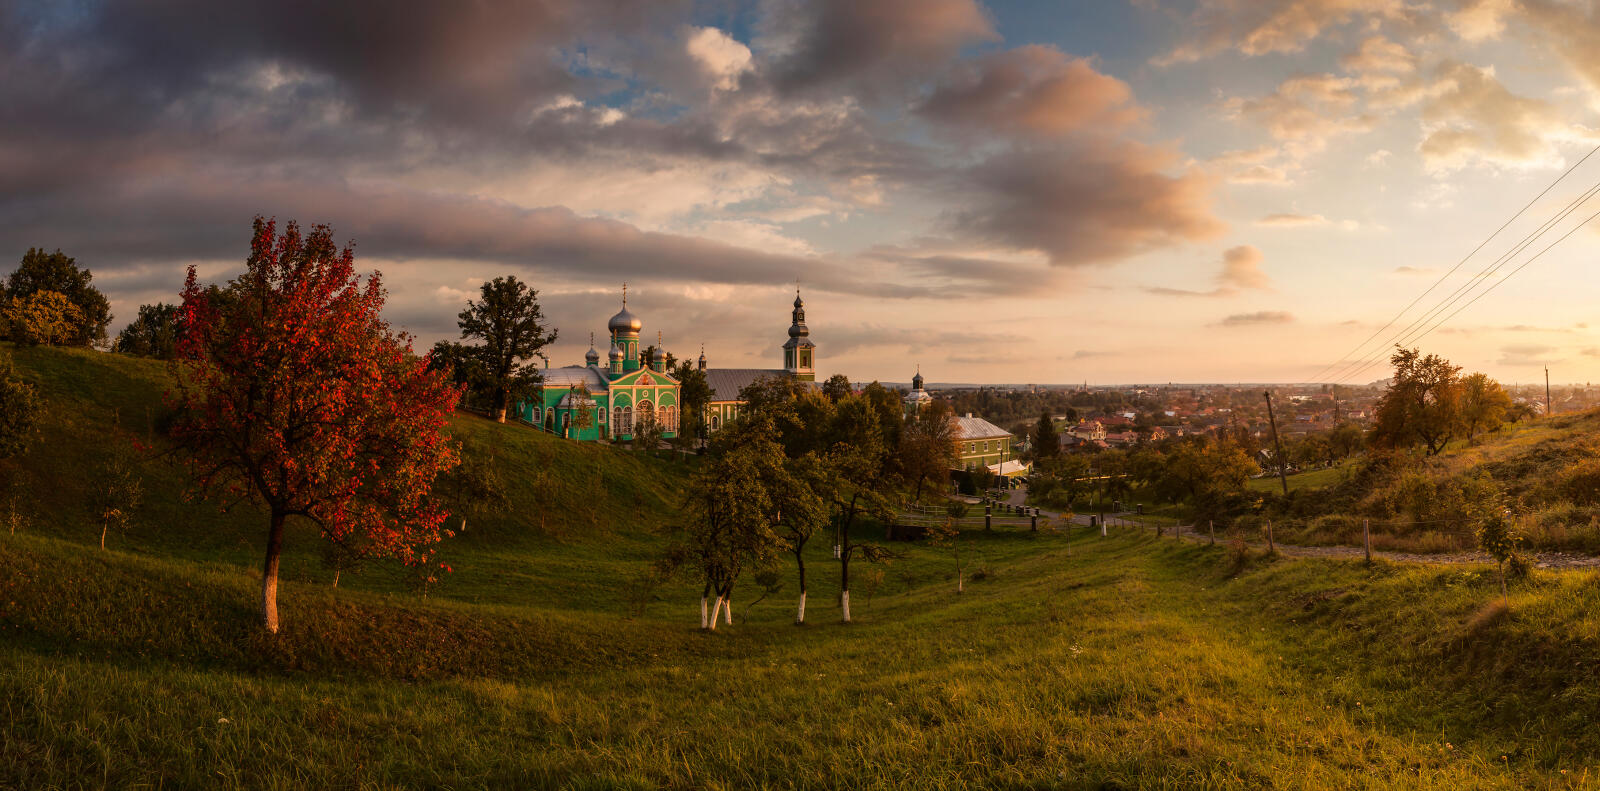
\includegraphics[width=\textwidth]{gtx_exp/zmonastery}
	\end{subfigure}~
	\begin{subfigure}[b]{0.32\textwidth}
		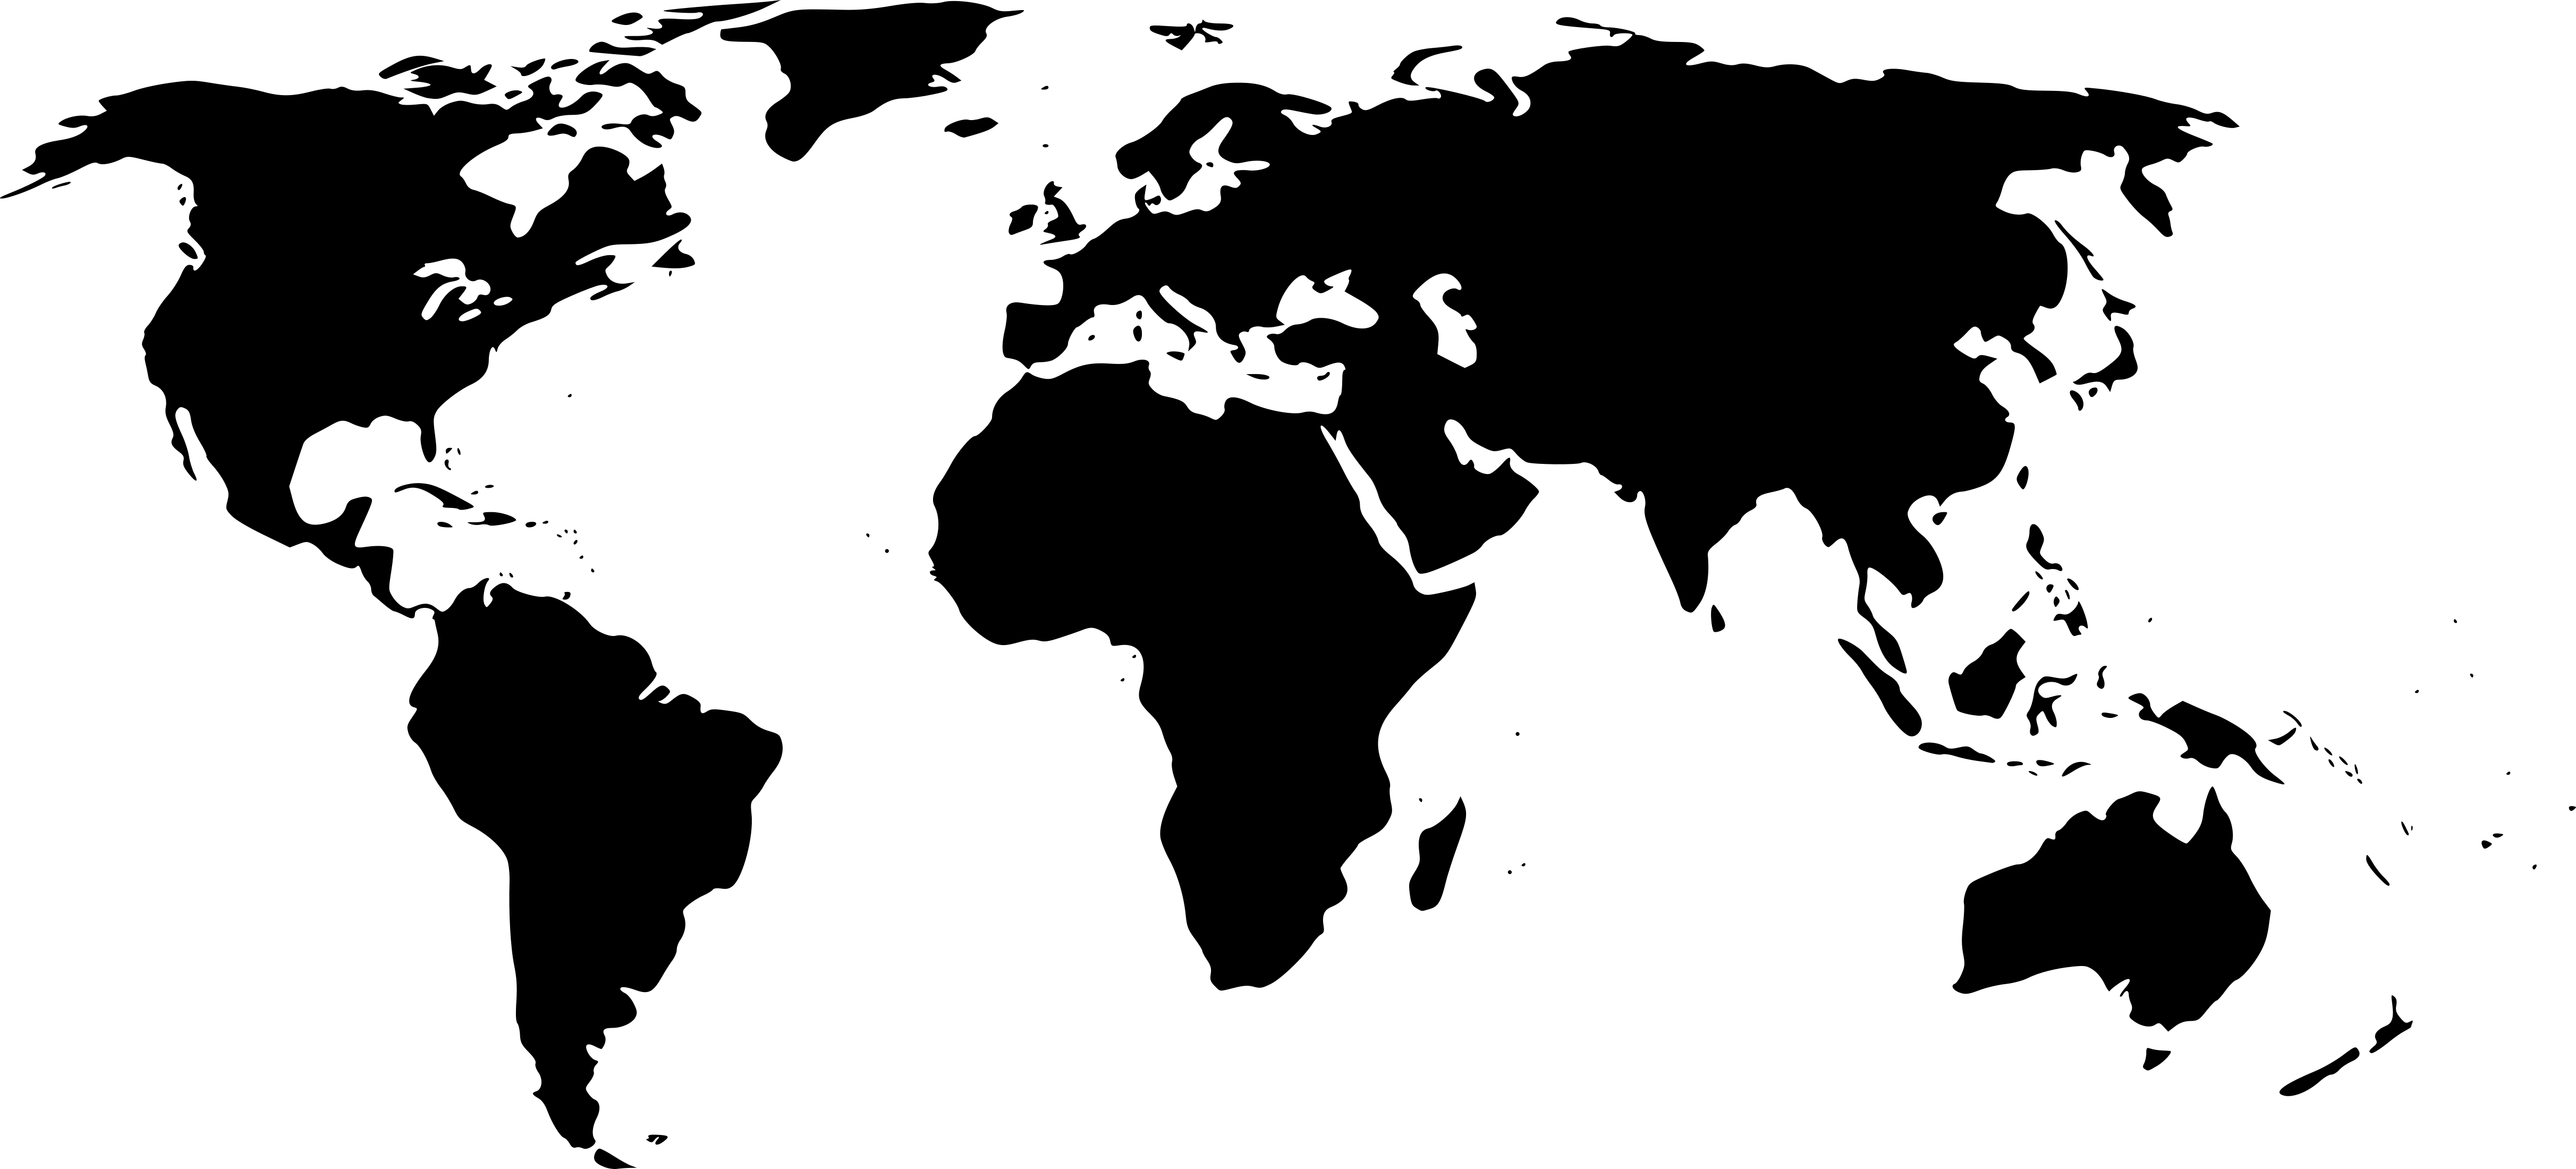
\includegraphics[width=\textwidth]{gtx_exp/zworld}
	\end{subfigure}~
	\begin{subfigure}[b]{0.32\textwidth}
		
\includegraphics[width=\textwidth]{gtx_exp/nips_poster}
	\end{subfigure}

	\begin{subfigure}[b]{0.32\textwidth}
		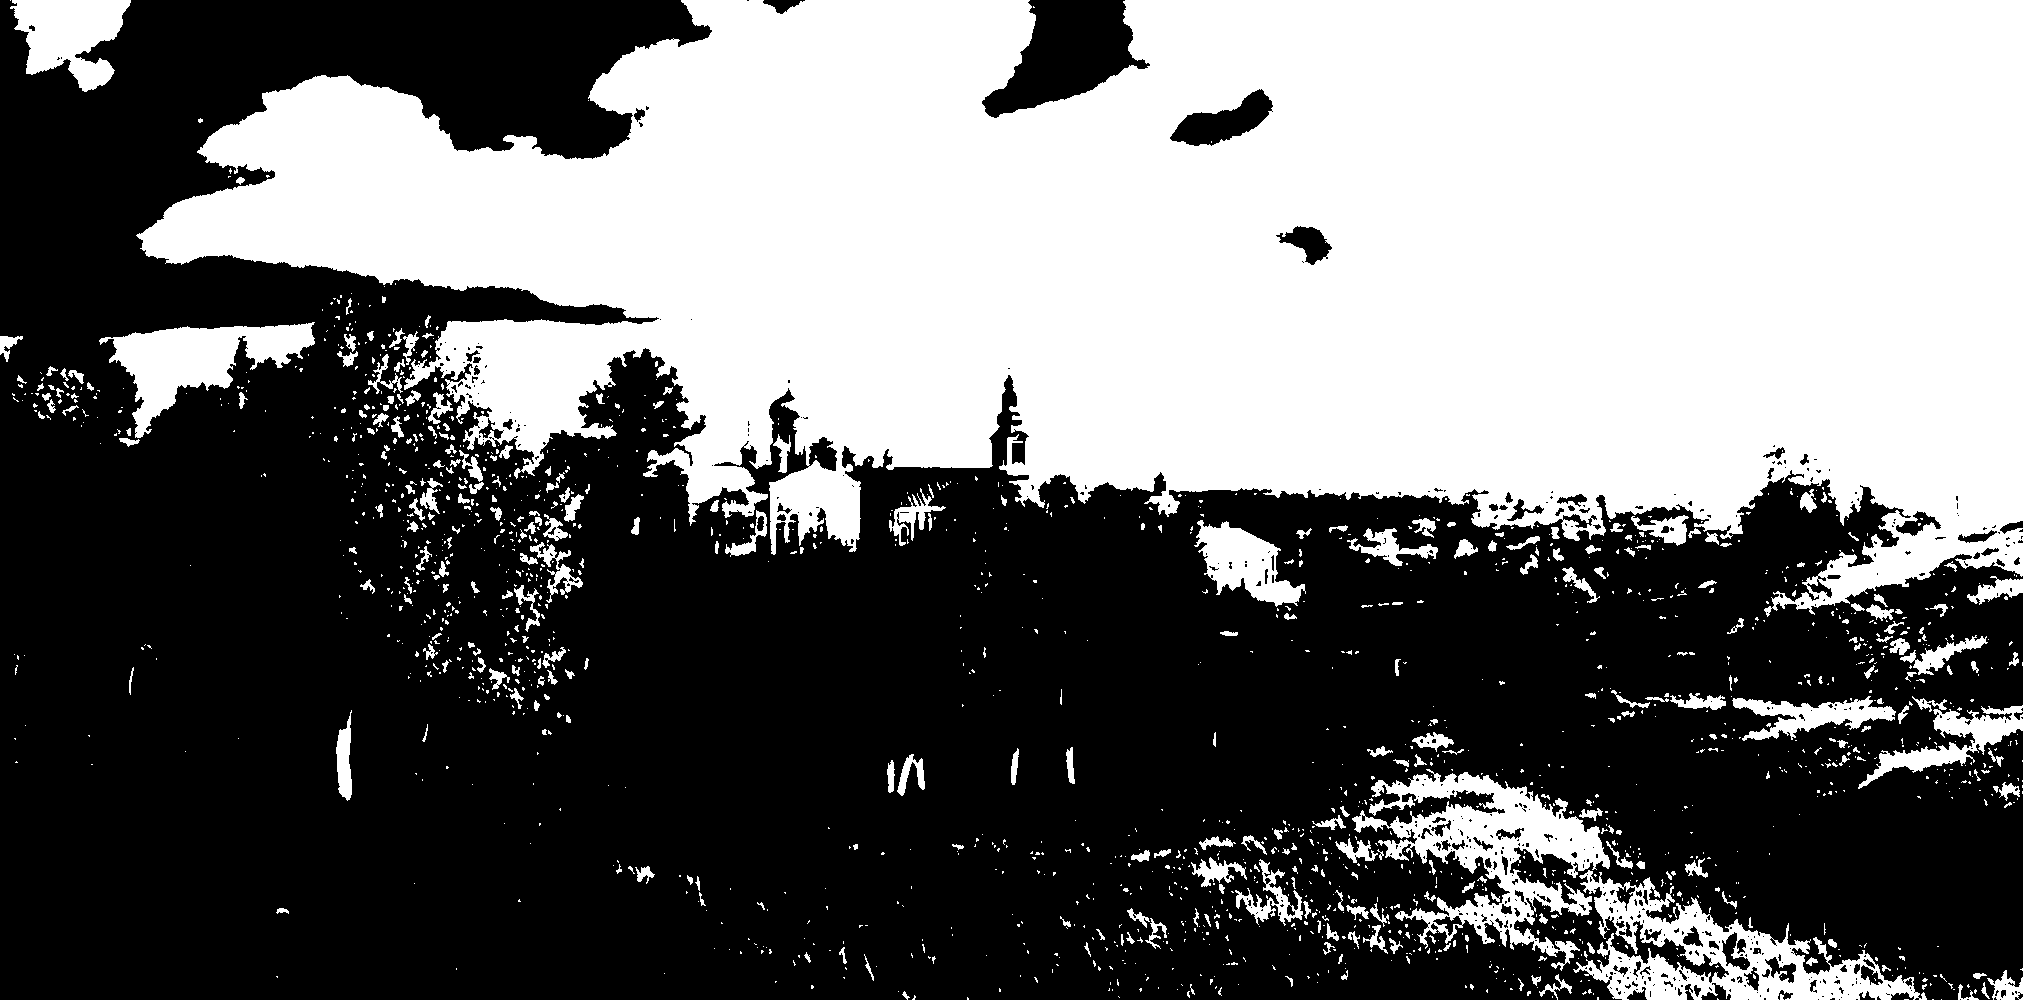
\includegraphics[width=\textwidth]{gtx_exp/zmonastery_bin}
		\caption{monastery}
	\end{subfigure}~
	\begin{subfigure}[b]{0.32\textwidth}
		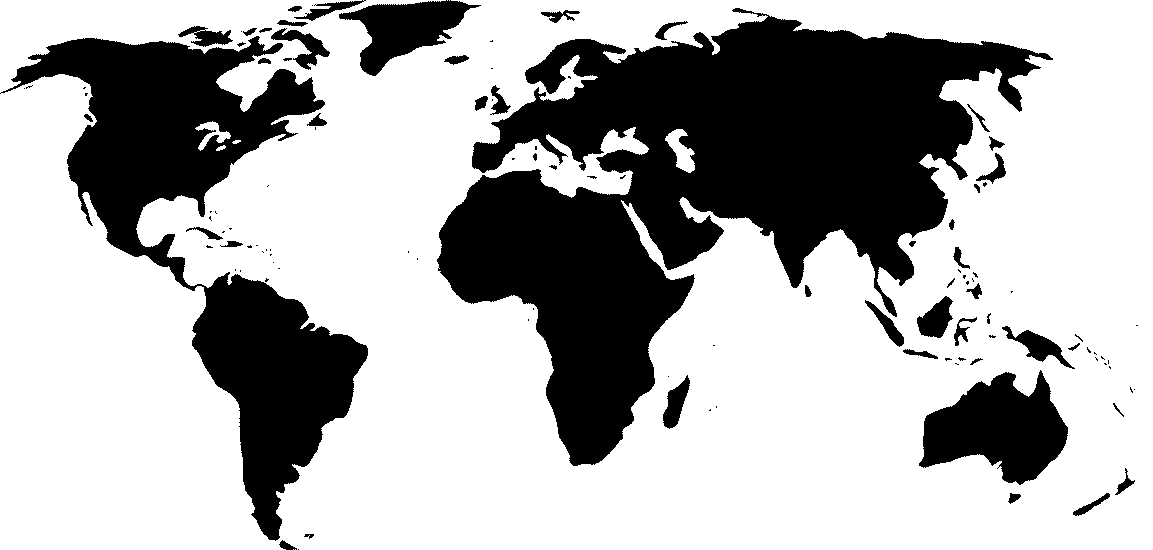
\includegraphics[width=\textwidth]{gtx_exp/zworld_bin}
		\caption{world}
	\end{subfigure}~
	\begin{subfigure}[b]{0.32\textwidth}
		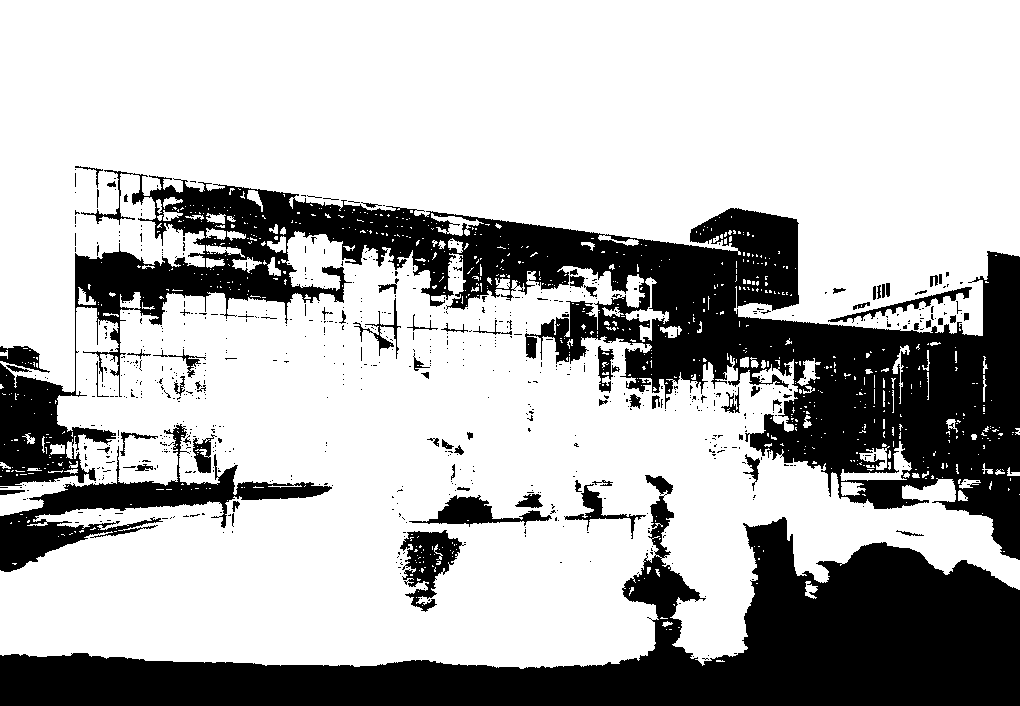
\includegraphics[width=\textwidth]{gtx_exp/nips_poster_bin}
		\caption{poster}
	\end{subfigure}

	\begin{subfigure}[b]{0.32\textwidth}
		
\includegraphics[width=\textwidth]{gtx_exp/nips_logo}
	\end{subfigure}~
	\begin{subfigure}[b]{0.32\textwidth}
		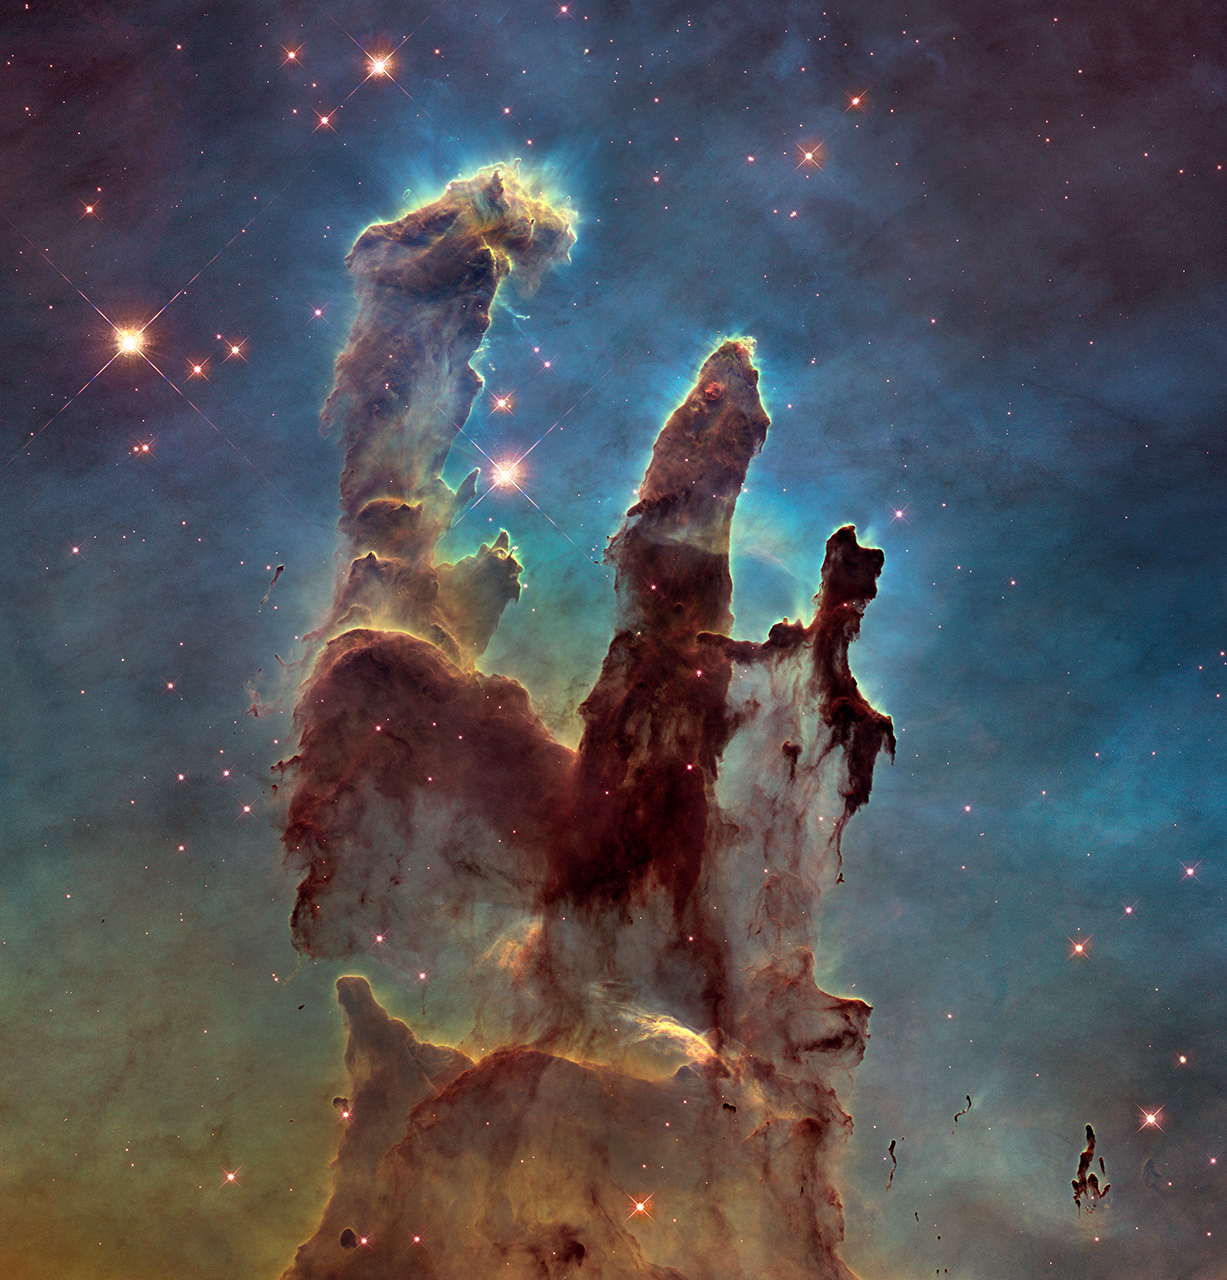
\includegraphics[width=\textwidth]{gtx_exp/space}
	\end{subfigure}~
	\begin{subfigure}[b]{0.32\textwidth}
		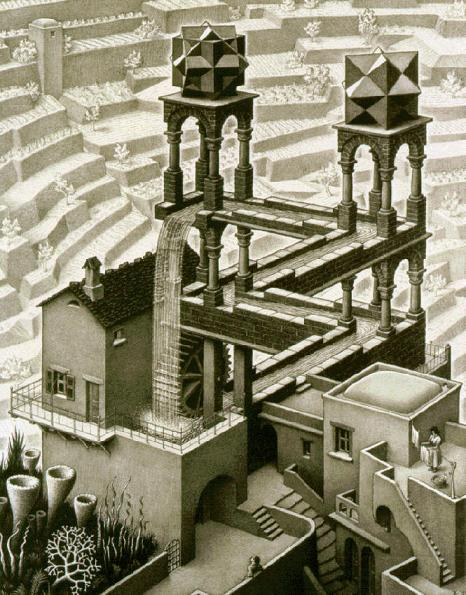
\includegraphics[width=\textwidth]{gtx_exp/waterfall}
	\end{subfigure}

	\begin{subfigure}[b]{0.32\textwidth}
		
\includegraphics[width=\textwidth]{gtx_exp/nips_logo_bin}
		\caption{logo}
	\end{subfigure}~
	\begin{subfigure}[b]{0.32\textwidth}
		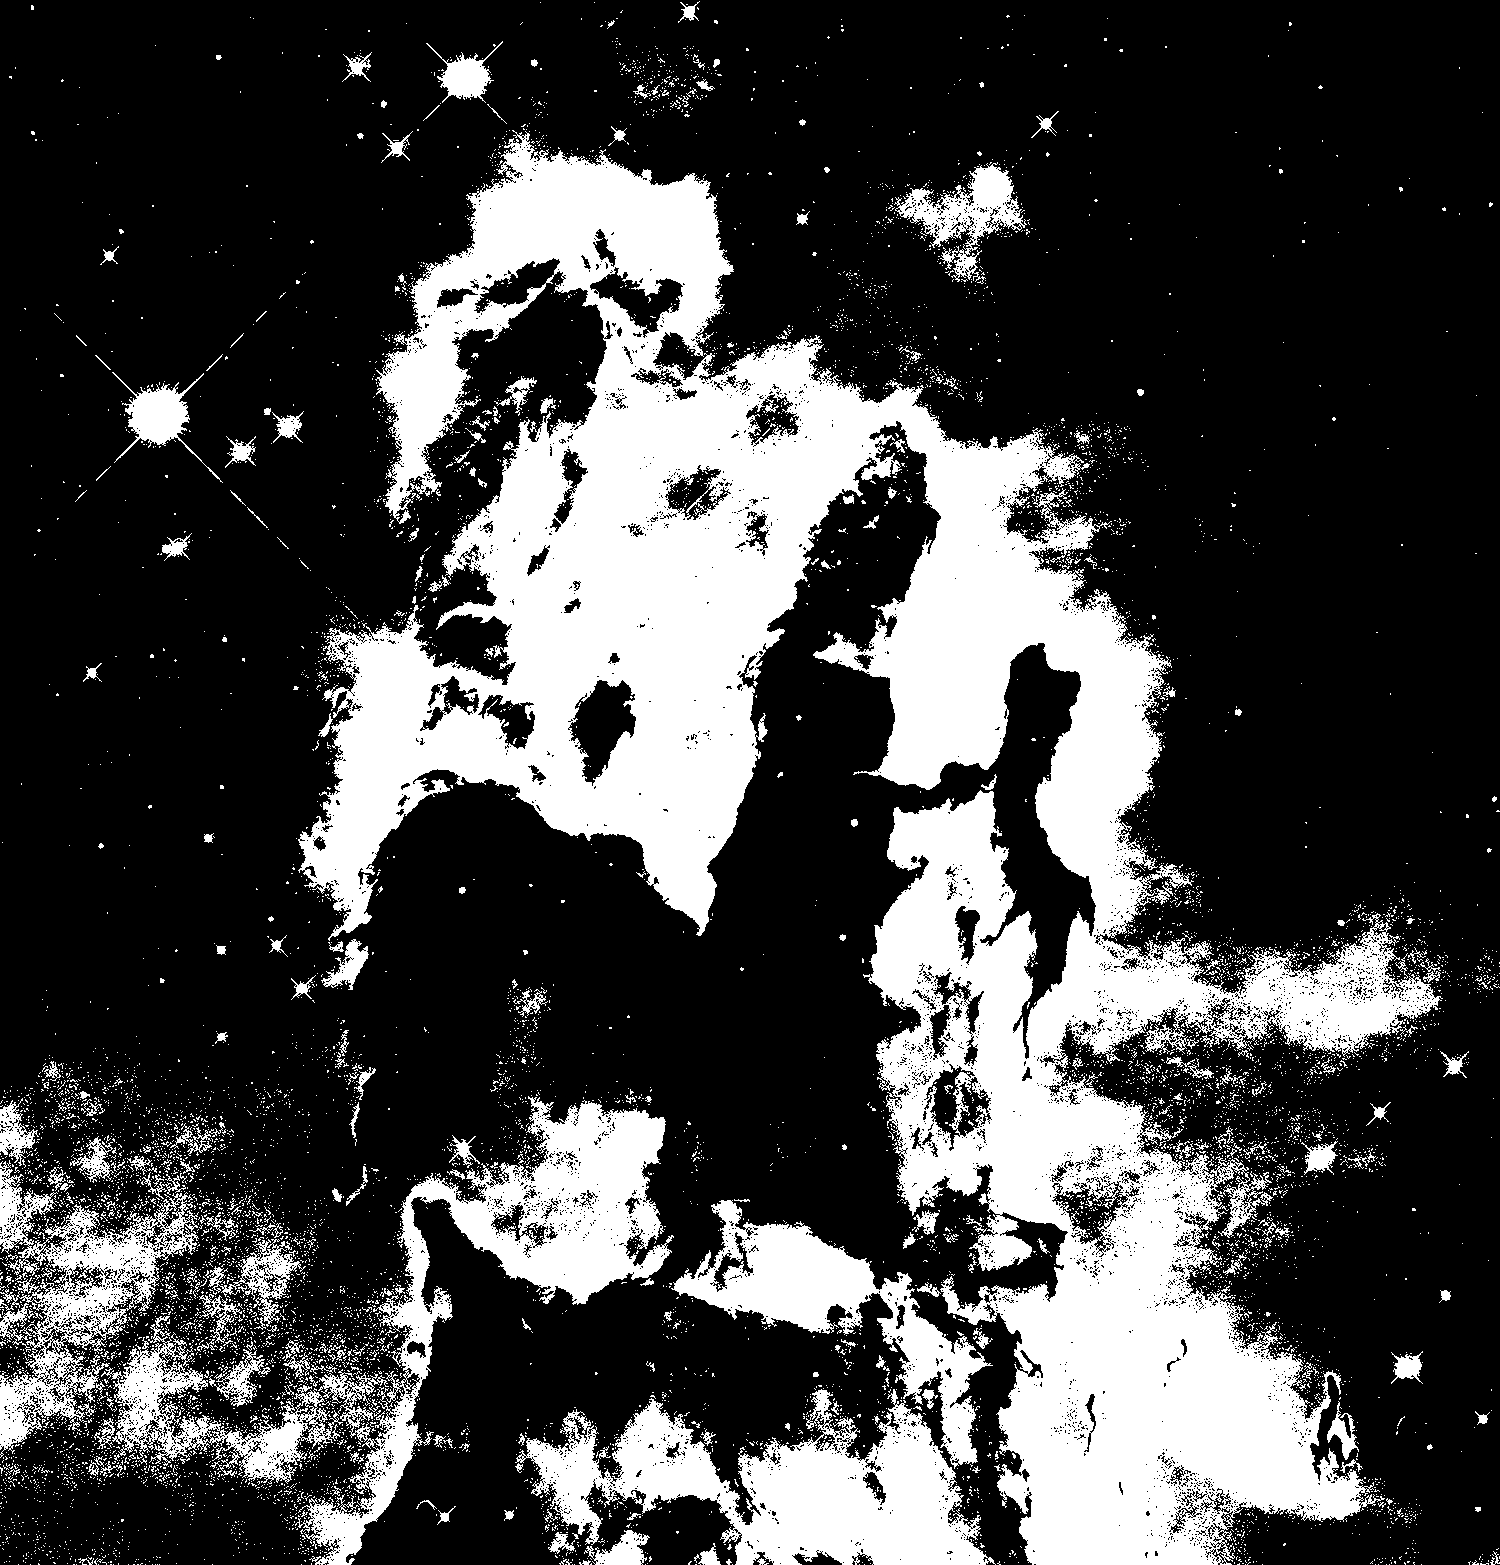
\includegraphics[width=\textwidth]{gtx_exp/space_bin}
		\caption{space}
	\end{subfigure}~
	\begin{subfigure}[b]{0.32\textwidth}
		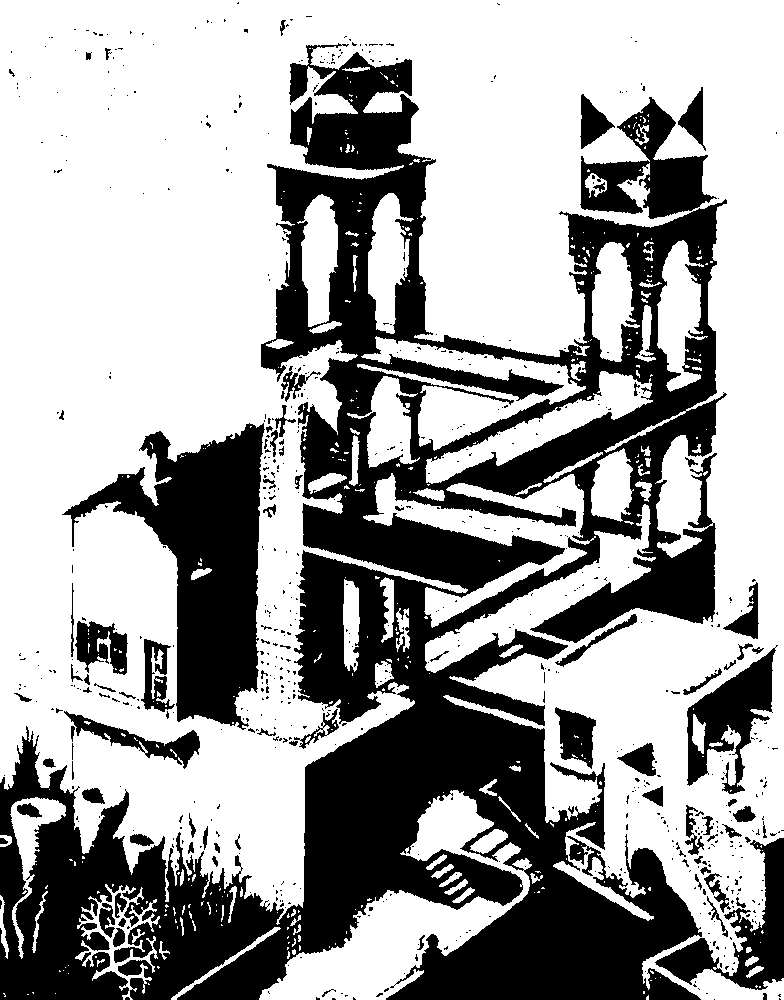
\includegraphics[width=\textwidth]{gtx_exp/waterfall_bin}
		\caption{waterfall}
	\end{subfigure}
	\caption{Real world pictures and their binarized version}\label{fig:gtx_xp_bwpics}
\end{figure}

\subsubsection{Stretch}

The first property of Galaxy trees we wish to evaluate is their stretch, which depends only of graph
topology. Recall that following equation~\autoref{eq:test_stretch_def}, we define the average test
edge stretch as $\frac{1}{|\etest{}|} \sum_{(u,v) \in \etest{}} |\mathrm{path}^T_{u,v}|$,
where $|\mathrm{path}^T_{u,v}|$ is the unique path between $u$ and $v$ in $T$.

As we consider unweighted graphs, we compare \gtx{} with a natural baseline, namely a spanning tree
rooted at the highest degree node and obtained through a breadth first visit of the graph. This
involves randomness in the order in which nodes are visited. Likewise in \gtx{}, the choice of the edge
linking two stars is not always unique, meaning that we have to break ties at random.  Therefore,
for each graph, we repeat the tree construction \np{12} times and present the average result, noting that
the variance (showed as error bar in \autoref{fig:gtx_xp_st}) is small.

On \lpa{} and \triangle{}, we see in \autoref{fig:gtx_xp_st} that both trees exhibits logarithmic stretch, although with a
larger constant for \gtx{}. Note that this is also the case for others low stretch tree methods
\autocite[Section 5.3.1]{papplow}. On \grid{} however, \gtx{} preserves this logarithmic stretch growth
while this is visually no longer the case for \bfs{}.
In that case, we cannot expect a better stretch than $\frac{\log n}{2048}$ according to
\autocite[Theorem 6.6]{LowerBound95}.

\begin{figure}[tbh]
	\centering
	\begin{subfigure}[b]{0.9\textwidth}
		\includegraphics[width=\textwidth]{gtx_exp/gridst}
		\caption{\grid{} }\label{fig:gtx_xp_gridst}
	\end{subfigure}

	\begin{subfigure}[b]{0.9\textwidth}
		\includegraphics[width=\textwidth]{gtx_exp/past}
		\caption{\lpa{} }\label{fig:gtx_xp_past}
	\end{subfigure}

	\begin{subfigure}[b]{0.9\textwidth}
		\includegraphics[width=\textwidth]{gtx_exp/trst}
		\caption{\triangle{} }\label{fig:gtx_xp_trst}
	\end{subfigure}
	\caption{Stretch over graphs of increasing size}\label{fig:gtx_xp_st}
\end{figure}

\subsubsection{Sign prediction}

The second design goal of Galaxy trees is to accurately predict the sign of edges in $\etest{}$.
Except for the three real datasets that already include signs\footnote{We nonetheless perform some
preprocessing in order to make them undirected and to remove the small proportion of conflicting edges
(e.g. positive from $u$ to $v$ but negative from $v$ to $u$).}, all the other are constructed,
meaning we have to set sign on their edges in the first place. This is done by partitioning the
nodes into two clusters. For \gplus{} we use node gender, for pictures we use node color (black or
white), and for all others, we propagate labels $0$ and $1$ from randomly selected high degree nodes.
Once each node belongs to one of the two clusters, we set the sign of an edge between two nodes to
be $+$ if they are in the same cluster and $-$ otherwise.  Predicting using path parity will thus
gives perfect result. To test performance in real situations, we then add noise, that
is we select a fraction of edges uniformly at random and flip their sign. 

Like in \autoref{s:exp}, we evaluate the performance of our prediction using the Matthews
Correlation Coefficient (MCC), defined in equation~\autoref{eq:troll_mcc} \vpageref{eq:troll_mcc}.
As showed in \autoref{fig:gtx_xp_mcc}, when the noise level is low, \gtx{} performs better than
\bfs{}. As the noise level gets higher, they have similar performance. Note also than in
\autoref{fig:gtx_xp_pasynthmcc}, \gtx{} is less sensible to the size of the graph.

\begin{figure}[tbh]
	\centering
	\begin{subfigure}[b]{0.47\textwidth}
		\includegraphics[width=\textwidth]{gtx_exp/grsynthmcc}
		\caption{Synthetic \grid{} }\label{fig:gtx_xp_grsynthmcc}
	\end{subfigure}~
	\begin{subfigure}[b]{0.47\textwidth}
		\includegraphics[width=\textwidth]{gtx_exp/grrwmcc}
		\caption{Pictures \grid{} }\label{fig:gtx_xp_grrwmcc}
	\end{subfigure}
	\begin{subfigure}[b]{0.47\textwidth}
		\includegraphics[width=\textwidth]{gtx_exp/pasynthmcc}
		\caption{Synthetic \lpa{} }\label{fig:gtx_xp_pasynthmcc}
	\end{subfigure}~
	\begin{subfigure}[b]{0.47\textwidth}
		\includegraphics[width=\textwidth]{gtx_exp/trmcc}
		\caption{\triangle{} }\label{fig:gtx_xp_trmcc}
	\end{subfigure}
	\begin{subfigure}[b]{0.47\textwidth}
		\includegraphics[width=\textwidth]{gtx_exp/parwmcc}
		\caption{Real world network }\label{fig:gtx_xp_parwmcc}
	\end{subfigure}
	\caption{MCC over various graphs}\label{fig:gtx_xp_mcc}
\end{figure}

To further assess the quality of our trees, we plug them in them into an existing heuristic method
to predict edge sign: \asym{}~\autocite{Kunegis2009}.
%\Todo{It might also be interesting to see if that would be a good training set for our troll method, although it has to be checked it makes sense from a running time point of view.}
It computes the exponential of the adjacency matrix after it has
been reduce to $z$ dimension. This allows to count the sign of all paths between two pairs of nodes
with decreasing weight depending of their length. To simulate an active learning setting, we reveal
only a subset of edge in $A$. This subset can be: $i)$ the edges forming a \bfs{}, $ii)$ the edges
forming a \gtx{} $iii)$ $|V|-1$ edges chosen uniformly at random.
We set the parameter $z$ equal to $15$ because $i)$ it is one of the best in \cite[Fig.
11]{Kunegis2009} and $ii)$ it performs well on real datasets in \cite[Fig.3]{Cesa-Bianchi2012a}.
% , and $iii)$ it was good in our initial testing (\texttt{20150401\_wed\_spectral.ipynb}).

As the \asym{} has a $O(n^3)$ complexity and uses quite some memory at prediction time, the larger
graphs used previously are not all included. The conclusion of \autoref{fig:gtx_xp_asym} is that
except on social networks, it is better to use spanning trees than random edges. Specifically, \gtx{}
on \grid{} and \bfs{} elsewhere.

\begin{figure}[tbh]
	\centering
	\begin{subfigure}[b]{0.47\textwidth}
		\includegraphics[width=\textwidth]{gtx_exp/grsynthasym}
		\caption{Synthetic \grid{} \label{fig:gtx_xp_grsynthasym}}
	\end{subfigure}~
	\begin{subfigure}[b]{0.47\textwidth}
		\includegraphics[width=\textwidth]{gtx_exp/grrwasym}
		\caption{\enquote{Real} \grid{} }\label{fig:gtx_xp_grrwasym}
	\end{subfigure}
	\begin{subfigure}[b]{0.47\textwidth}
		\includegraphics[width=\textwidth]{gtx_exp/pasynthasym}
		\caption{Synthetic \lpa{} }\label{fig:gtx_xp_pasynthasym}
	\end{subfigure}~
	\begin{subfigure}[b]{0.47\textwidth}
		\includegraphics[width=\textwidth]{gtx_exp/trasym}
		\caption{\triangle{} }\label{fig:gtx_xp_trasym}
	\end{subfigure}
	\begin{subfigure}[b]{0.47\textwidth}
		\includegraphics[width=\textwidth]{gtx_exp/parwasym}
		\caption{Real world network }\label{fig:gtx_xp_parwasym}
	\end{subfigure}
	\caption{\asym{} over various graphs}\label{fig:gtx_xp_asym}
\end{figure}

\iffalse
Finally\marginpars{Actually I never did it because \shz{} wasn't implemented at the time, so now is
a good occasion}\todo*{Run shazoo on galaxy tree} we also compare \gtx{} with \bfs{} and \rst{} on
the task of nodes prediction using \shz{} algorithm~\autocite{Vitale2012}.
\fi


\section{Conclusion}


\begingroup
\small
\setstretch{0.9}
\todos

\setlength\bibitemsep{2pt}
\printbibliography
\endgroup

% \bibliography{/home/orphee/data/projects/biblio/library.bib,more.bib}
% \bibliographystyle{plainnat}
\end{document}
